\documentclass[border=10pt]{standalone}
\usepackage{pgfplots}
\usepackage{pgfplotstable}
\pgfplotsset{width=7cm,compat=1.8}
\begin{document}
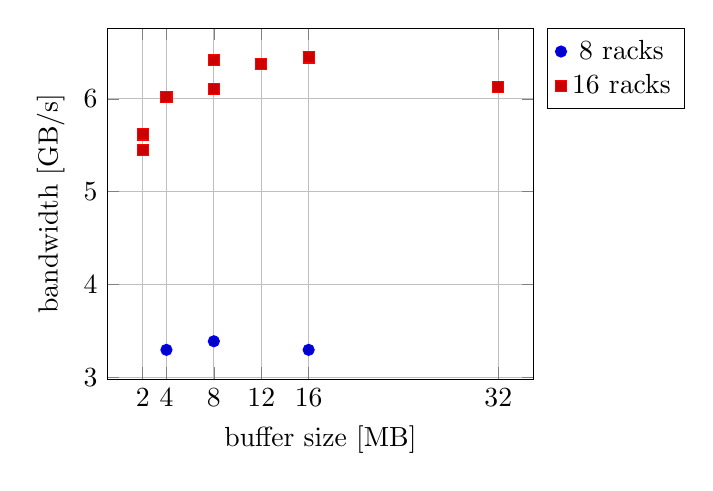
\begin{tikzpicture}
\begin{axis}[
    %title=Measured bandwidth,
    xlabel={buffer size [MB]},
    ylabel={bandwidth [GB/s]},
    xtick={2,4,8,12,16,32},
    xticklabels={2,4,8,12,16,32},
    grid=major,
    legend entries={8 racks, 16 racks},
    legend pos = outer north east,
]
\addplot+[only marks] plot coordinates {
	(4,2.74784189/20*24)
	(8,2.8248482018/20*24) 
  	(16,2.74784189/20*24)};
\addplot+[only marks] plot coordinates {
	(2,4.5439519159/20*24)
	(2,4.6800686629/20*24) 
  	(4,5.0196030561/20*24)
  	(8,5.0909090909/20*24)
  	(8,5.3481843146/20*24)
  	(12,5.3111982543/20*24)
  	(16,5.3706242488/20*24)
  	(32,5.1029851666/20*24)};
\end{axis}
\end{tikzpicture}
\end{document}